%\setmarginsrb{3 cm}{2.5 cm}{3 cm}{2.5 cm}{1 cm}{1.5 cm}{1 cm}{1.5 cm}
\documentclass[11pt,a4paper]{article}
%\documentclass[paper=a4, fontsize=15pt]{article}
\usepackage{gensymb}
\usepackage{amsmath}
\usepackage{stackrel}
\usepackage[utf8]{inputenc}
\usepackage{anysize}
%\marginsize{2cm}{2cm}{2cm}{2cm} % Izquierda, derecha, arriba, abajo
\usepackage{titletoc}
\usepackage[T1]{fontenc}
\usepackage{textcomp}
\usepackage{sectsty}
\usepackage[small]{titlesec}
\usepackage[spanish]{babel}
\usepackage{graphicx}
\usepackage{hyperref}
\usepackage[utf8]{inputenc}
\usepackage[usenames, dvipsnames]{color}
\usepackage{verbatim} 
\usepackage{multicol}
\usepackage{multirow} % para las tablas
\usepackage{amsmath}
\usepackage{caption}
\usepackage{subcaption}
\usepackage{array}
\usepackage{float}
\usepackage[numbers]{natbib} 
\usepackage{color} 
\usepackage{listings}
\usepackage{hyperref}

\providecommand{\abs}[1]{\lvert#1\rvert}
\providecommand{\norm}[1]{\lVert#1\rVert}
\hypersetup{
    colorlinks=true,
    linkcolor=blue,
    filecolor=magenta,
    citecolor=blue,
    urlcolor=cyan,
}
%\hypersetup{colorlinks,linkcolor={blue},citecolor={blue},urlcolor={red}}  
\urlstyle{same}
\usepackage{enumerate}
\newcommand\tab[1][1cm]{\hspace*{#1}}
\newcommand{\grad}{$^{\circ}$}


% Para agregar encabezado y pie de página
\usepackage{fancyhdr} 
\pagestyle{fancy}
\fancyhf{}
\lhead{
\includegraphics[width=1.25cm]{images/EPIE.jpeg} \footnotesize Software de Telecomunicaciones}
\rhead{
\includegraphics[width=1cm]{images/ucsm.png}}
\fancyfoot[R]{\thepage}

\usepackage{listings} % Para usar código fuente
\lstset{
    %language=Java,
    keywords={break,case,catch,continue,else,elseif,end,for,function,       global,if,otherwise,persistent,return,switch,try,while},
    basicstyle=\scriptsize,
    frame=tb, % draw a frame at the top and bottom of the code block
    tabsize=4, % tab space width
    showstringspaces=false, % don't mark spaces in strings
    numbers=left, % display line numbers on the left
    numberstyle=\tiny\color{gray},
    commentstyle=\color{green}, % comment color
    keywordstyle=\color{blue}, % keyword color
    stringstyle=\color{red} % string color
    basicstyle=\ttfamily,
    columns=fullflexible,
    frame=single,
    breaklines=true,
    postbreak=\mbox{\textcolor{red}{$\hookrightarrow$}\space},
    %title=\lstname
}
\lstdefinestyle{python}
{language=python,
}
\lstset{
        tabsize=2,
        backgroundcolor=\color[HTML]{F0F0F0}, 
        captionpos=b, 
        basicstyle=\footnotesize\ttfamily, 
        columns=fixed, 
        extendedchars=true, 
        breaklines=true, 
        prebreak = \raisebox{0ex}[0ex][0ex]{\ensuremath{\hookleftarrow}},
        showtabs=false,
        showspaces=false, 
        keywordstyle=\bfseries\color[HTML]{007020}, 
        commentstyle=\itshape\color[HTML]{60A0B0},
        stringstyle=\color[HTML]{4070A0},
}

\lstset{language=Matlab,%
    %basicstyle=\color{red},
    breaklines=true,%
    morekeywords={matlab2tikz},
    keywordstyle=\color{blue},%
    morekeywords=[2]{1}, keywordstyle=[2]{\color{black}},
    identifierstyle=\color{black},%
    stringstyle=\color{mylilas},
    commentstyle=\color{mygreen},%
    showstringspaces=false,%without this there will be a symbol in the places where there is a space
    numbers=left,%
    numberstyle={\tiny \color{black}},% size of the numbers
    numbersep=9pt, % this defines how far the numbers are from the text
    emph=[1]{for,end,break},emphstyle=[1]\color{red}, %some words to emphasise
    %emph=[2]{word1,word2}, emphstyle=[2]{style},    
}


\begin{document}
\renewcommand{\refname}{BIBLIOGRAFÍA}


\begin{titlepage}
		\newcommand{\HRule}{\rule{\linewidth}{0.5mm}}
		\center 
		
\includegraphics[scale=0.5]{images/ucsm.png}\\[1cm]
		\textsc{\LARGE Software de Telecomunicaciones}\\[0.5cm]  
		
		\HRule \\[0.5cm]
		{\huge \bfseries 4NEC2}\\[0.5cm]
		
		\HRule \\[0.5cm]
		
		\begin{minipage}{0.5\textwidth}
		\begin{flushleft} \large
			\emph{Docente:}\\
			Ing. Mario W. Urrutia Espinoza\\
            Escuela P. Ingeniería Electrónica\\
		\end{flushleft}
			\end{minipage}~
			\begin{minipage}{0.4\textwidth}
            
		\begin{flushright} \large
			\emph{Autor:} \\
			Medina Madueño, Paúl M.\\
		\end{flushright}
     
	\end{minipage}\\[2 cm]
		\vfill 
\end{titlepage}
\thinspace
\tableofcontents
\listoffigures
\newpage

%\thinspace

\section{Objetivos del programa}
\begin{itemize}
    \item Tiene como principal objetivo el apoyo como herramienta para poder diseñar una antena sin la necesidad del uso de diferentes equipos de alto costo, y los resultados obtenidos son muy semejantes al de la realidad.
    \item Se puede usar este tipo de simuladores desde la comodidad de nuestro hogar sin la necesidad de emplear laboratorios, y es una soluci\'on optima para poder orientar al alumno a seguir conociendo m\'as sobre las antenas que existen.
    \item Como se ver\'a a lo largo de este documento, el uso de este software es una herramienta muy importante y lo mejor es que ees libre, lo que significa que no se paga ninguna licencia.
\end{itemize}


 \section{Introducci\'on}\label{sec:1}
 
 NEC(\textit{Numerical Electromagnetic Code}) es un programa utilizado para la representación de las propiedades electromagnéticas de las antenas u otras estructuras metálicas  \cite{ant} . Esta basado en las solución num\'erica de las ecuaciones integrales para corrientes inducidas en la estructura de una antena para fuentes y campos auxiliares \cite{moron} ,  su interfaz gr\'afica es 4NEC2.\\

4NEC2 es un software con m\'ultiples ventanas que nos posibilita un diseño completo y bien estructurado de una antena o en su defecto una l\'inea de transmisi\'on \cite{Gallardo} .\\

En este software tenemos la posibilidad de ingresar datos por un editor de textos y con el m\'inimo conocimiento de los comandos de NEC podemos construir una estructura \cite{Miron} ,  ya que en la actualidad , NEC sigue siendo el coraz\'on de esta aplicaci\'on.\\

\section{Interfaz de Usuario para 4NEC2}\label{sec:2}
En este apartado explicaremos 4 de las m\'ultiples ventanas con las respectivas teclas que están en par\'entesis, que son su manera de entrar a ellas de manera mas r\'apida:

\begin{itemize}
    \item Main(F2)
    \item Geometry(F3)
    \item Pattern(F4)
    \item Impedance(F5)
\end{itemize}

\subsection{Main (F2)}\label{sec:2.1}

En esta ventana podemos observar los datos generales obtenidos de los archivos de entrada y salida, teniendo la opci\'on de poder generar patrones de campo ya sean lejanos o cercanos. Todo esto se ve en la siguiente figura.

\begin{figure}[H]
    \centering
    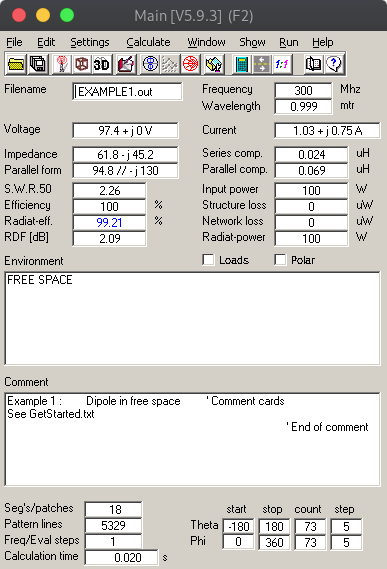
\includegraphics[scale=0.35]{images/Interfaz/main.png}
    \caption{Main}
    \label{fig1:Main}
\end{figure}

\subsection{Geometry (F3)}\label{sec:2.2}

Aqui se muestra la estructura geométrica donde también se puede incluir las fuentes, l\'ineas de transmisíon y cargas. El programa no es muy sofisticado ya que fue desarrollado inicialmente para diseñar estructuras met\'alicas geom\'etricas \cite{ant} .

\begin{figure}[H]
    \centering
    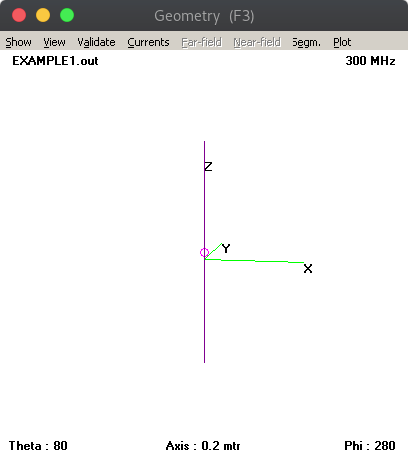
\includegraphics[scale=0.45]{images/Interfaz/geometry.png}
    \caption{Geometry}
    \label{fig2:Geometry}
\end{figure}

\subsection{Pattern (F4)}\label{sec:2.3}

En esta ventana podemos ver el patr\'on de radiaci\'on de nuestra antena que se representan por defecto en coordenadas polares, como se ve en la siguiente figura.

\begin{figure}[H]
    \centering
    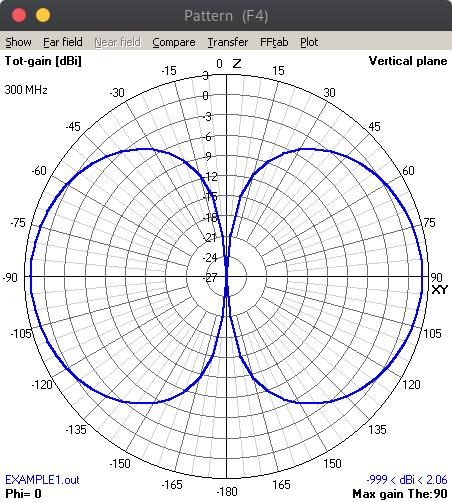
\includegraphics[scale=0.35]{images/Interfaz/pattern.png}
    \caption{Pattern}
    \label{fig3:Pattern}
\end{figure}

\subsection{Impedance(F5)}\label{sec:2.4}

Aquí podemos visualizar las gráficas de la $Z_{in}$, SWR, y si se determina la ganancia también se ve la relaci\'on de la frecuencia de entrada por medio de barridos front-to-back  \cite{ant} .

\begin{figure}[H]
    \centering
    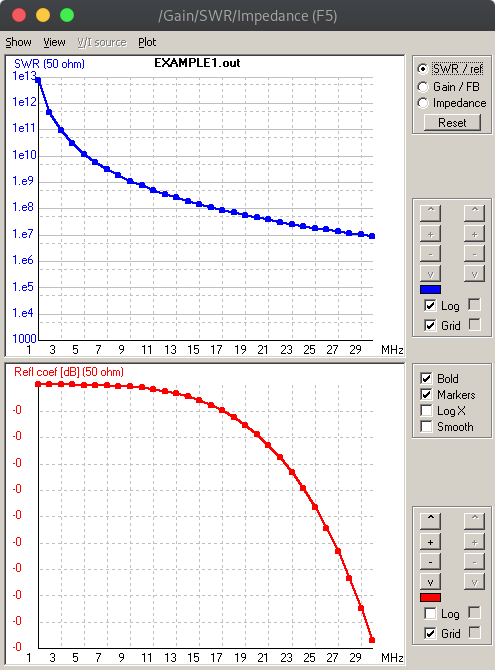
\includegraphics[scale=0.35]{images/Interfaz/impedancia.png}
    \caption{Impedance}
    \label{fig4:Impedance}
\end{figure}

\subsection{Otras ventanas que se pueden apreciar} \label{secc:2.5}

\begin{itemize}
    \item Carta de smith: Como otra herramienta tenemos la carta de smith donde podremos cer como se graf\'ica la impedancia y el ROE(SWR) con las atenuaciones y dem\'as par\'ametros.
    \item 3D Viewer: En esta ventana podremos observar tanto la antena como el patr\'on de radiaci\'on en 3D y cual ser\'a el campo afectado, adem\'as de la direcci\'on del patr\'on.
\end{itemize}

\section{Procesado}\label{sec:3}
En la interfaz 4NEC2 tenemos 4 modelados para poder diseñar nuestro proyecto, los cuales se pasar\'an a explicar.

\subsection{Modelado de la antena Geometry Edit}\label{sec:3.1}
Aquí se establece la estructura geométrica de la antena. Se ingresa en este modo entrando en la ventana main, en settings, y le damos a la opción de "Geometry edit", ahora ya podemos empezar con el modelado :
\begin{itemize}
    \item Especificar la frecuencia
    \item Añadir hilos
    \item Agregar una fuente
    \item Conductividad de los hilos
    \item Desplazar/voltear/escalar la antena
    \item Determinación de los parámetros de la tierra
\end{itemize}

\begin{figure}[H]
    \centering
    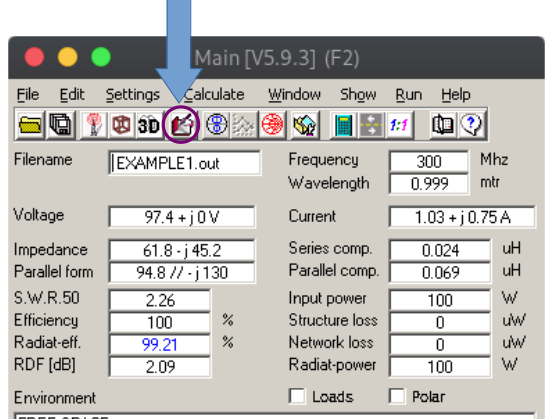
\includegraphics[scale=0.35]{images/Procesado/main2.png}
    \caption{Selección de par\'ametros de la antena}
    \label{fig4:parametros}
\end{figure}

Ahora bien dándole click a esta opción podemos visualizar la siguiente ventana donde nosotros ya podremos diseñar el modelo de nuestra antena.\\
Donde nosotros podremos ingresar los parámetros que deseamos darle a nuestro diseño además de la forma de la siguiente manera.

\begin{figure}[H]
    \centering
    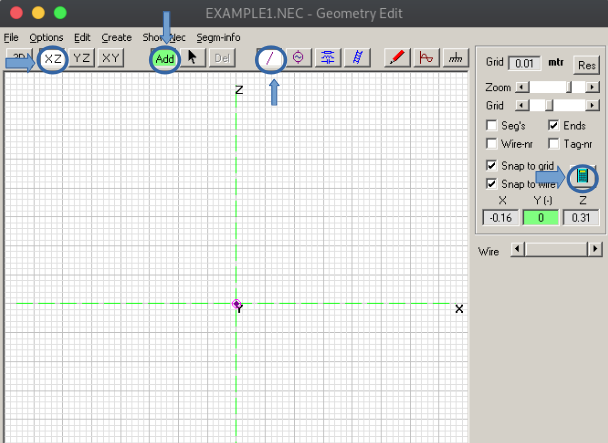
\includegraphics[scale=0.30]{images/4NEC2/geometry2.png}
    \caption{Análisis de la ventana de Geometry edit}
    \label{fig5:edit}
\end{figure}

Aqui podemos ver que se remarcaron 4 secciones donde:

\begin{itemize}
    \item XZ: es donde nosotros podemos graficar en 2D en la región de X y Z, también podemos cambiar como se puede apreciar en la imagen a diferente planos y por ultimo podremos visualizar la antena entera en el plano 3D que también esta como una opción en esta sección.
    \item ADD: con esta opción nosotros podremos añadir diferentes componentes ya sean fuentes, hilos, cargas RLC o lineas de transmisiones y también tenemos la opción de borrar lo ue deseamos con el botón "DEL", o movernos por el plano con la flecha ue se encuentra a su lado.
    \item En el siguiente sector de la barra de herramientas podemos ver que están los componentes que deseamos agregar con "ADD".
    \item La calculadora nos bota los datos deseados que vamos a tocar a lo largo del documento especificando cada uno de ellos.
    \item Un sector que no se marco, tiene la misma importancia ya que aquí podemos ingresar los datos de la frecuencia, los daros de la GND, y también podemos comentar el diseño de nuestra antena. Este segmento se encuentra a lado derecho del segmento de los componentes.
\end{itemize}

\subsection{Verificación del modelo}\label{sec:3.2}
Para comprobar los resultados tenemos 4 posibilidades, primero debemos fijarnos en el patrón de radiación de la antena, posteriormente debemos mirar la eficiencia de la estructura de la antena, la cual no puede ser mayor al 100\%, si se diera el caso sabremos que la simulación es incorrecta, debemos tener en cuenta que si nuestro modelo no tiene carga la eficiencia sera del 100\% ya que no tendrá perdidas,por otro lado si la eficiencia de nuestra antena esta por debajo del 50\% es muy probable que nuestros resultados sean incorrectos.\\
Como tercer paso debemos comprobar la impedancia de la antena, donde dbemos obtener un valor razonable, un valor realista, el punto más importante para saber si los resultados son acertados es la observación de la distribución de la energía. Se debe mirar el valor y la fase de la energía en cada segmento. Con estos conocimientos sobre el dipolo $\lambda/2$ está claro que los resultados son correctos .\\

\subsection{Modelado de una antena usando el notePAD editor}\label{sec:3.3}
En este modelado encontramos unas instrucciones básicas que necesitamos conocer antes de realizar nuestro diseño en este modelo los cuales son:
\begin{itemize}
    \item CM(comment - comentario): donde los primeros 30 caracteres son considerados como título.
    \item CE(fin de los comentarios)
    \item SY(variables): Para definir las variables de nuestro diseño
    \item GW(Geometry wire)
    \item GE(Geometry end)
    \item EX(excitation - excitación): Aquí definimos las fuentes de alimentación.
    \item FR(Frecuency - frecuencia): Aquí indicamos la frecuencia de trabajo.
    \item GN(Ground - Tierra): Definimos la caracterista de la tierra.
    \item LD(Load - Carga)
    \item TL(Transmission line - lineas de transmisión)
    \item NE(Near Electric Field - Campo eléctrico cercano)
    \item EN(End - Fín)
\end{itemize}

\subsection{NEC ecitor(old)}\label{sec:3.4}
En este editor si bien no tenemos ciertos datos predefinidos nosotros podemos colocarlos y en caso de hacer alg\'un cambio de cualquier componente podremos observar de cual se trata debido a que el componente a reemplazar o modificar se va resaltar en la ventana Geometry(F3), asi estaremos seguros de los cambios a realizar.

\subsection{NEC editor(new)}\label{sec:3.5}
A diferencia de otros este modelado se encuentra disponible solo en 4NEC2, y tiene un parecido a una tabla de excel, como se puede notar ya viene con ciertos valores los cuales se podr\'an modificar a gusto del diseñador, tiene diferentes pestañas para poder organizar mejor la informaci\'on de nuestro proyecto a realizar.

\section{Aplicaciones de 4NEC2}\label{sec:4}

Las aplicaciones de este programa son esencialmente para el diseño de antenas y el comportamiento de estas en un ambiente determinado, esta dirigido para la rama de ingeniería de telecomunicaciones, ya que se necesita conocimiento de electromagnetismo y lineas de transmisión para poder entender de donde vienen los datos obtenidos en las ventanas y entender a su vez si es correcto los resultados y si es factible el diseño de la antena, cabe resaltar que este es un programa hecho en casa por lo que puede tener unos errores.\\
Explorando un poco los archivos que ya tenemos en nuestro software podemos entender que podemos hacer una gran cantidad de antenas y proyectos, ya que nos permite variar las frecuencias de trabajo y la longitud de onda.

\section{Ejemplo de diseño de una antena Yagi}\label{sec:5}
Se hará el modelado de una antena Yagui con una frecuencia de 30 MHz y una longitud de onda de 10m aproximadamente.se vera como se coloca la frecuencia en la siguiente imagen.

\begin{figure}[H]
    \centering
    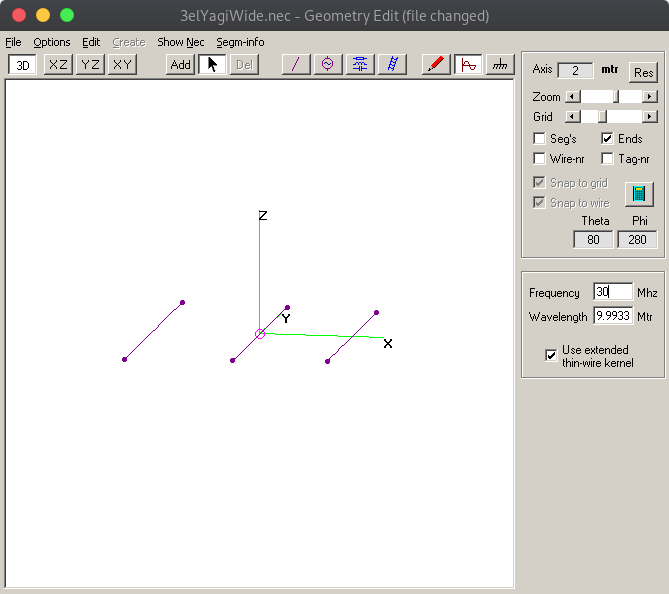
\includegraphics[scale=0.35]{images/Ejemplos/yagi.png}
    \caption{Antena Yagui en 3D}
    \label{fig3:yagui3d}
\end{figure}


\begin{figure}[H]
    \centering
    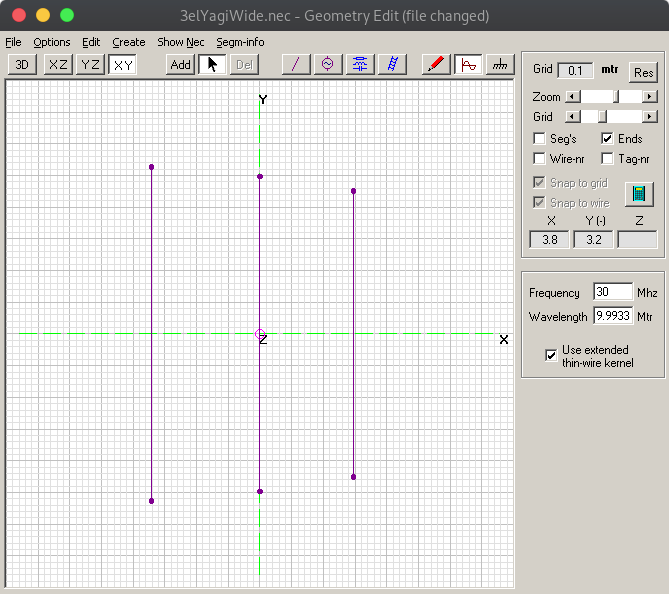
\includegraphics[scale=0.35]{images/Ejemplos/yagi1.png}
    \caption{Antena Yagui en 2D colocando par\'ametros}
    \label{fig3:yagui2d}
\end{figure}

En las imágenes anteriores nos damos cuenta que la longitud de onda es de aproximadamente 10m, ya que el programa mismo nos da el valor de la longitud de onda de manera automática a la hora de colocar la frecuencia de trabajo.

\begin{figure}[H]
    \centering
    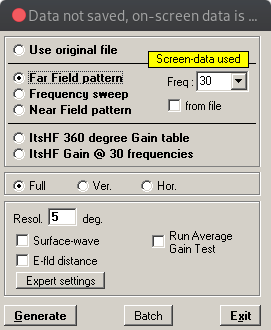
\includegraphics[scale=0.50]{images/Ejemplos/datos.png}
    \caption{Selección de datos de nuestro diseño}
    \label{fig3:yagui2d}
\end{figure}

En la imagen anterior podemos ver que tenemos múltiples opciones a elegir cada uno tiene una función especifica, la que usaremos ahora es la opción de "Far Field Pattern" la cual nos proporcionara los datos de su campo de irradiación, sus datos en la ventana de main, incluso podemos ver su resultado en la carta de smith como se demostrara en las siguientes imágenes.

\begin{figure}[H]
    \centering
    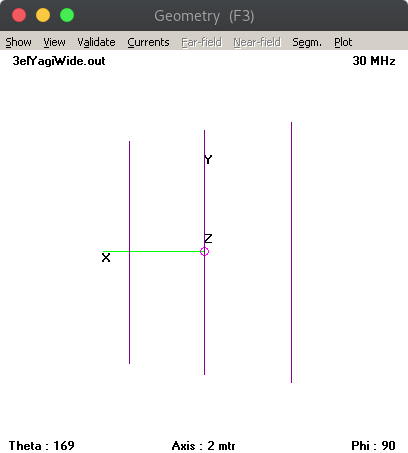
\includegraphics[scale=0.5]{images/Ejemplos/geo.png}
    \caption{Visualización de nuestra antena Yagui en geometry edit}
    \label{fig3:yagui2d}
\end{figure}

\begin{figure}[H]
    \centering
    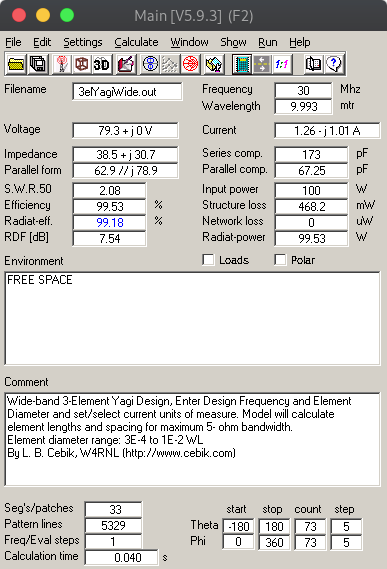
\includegraphics[scale=0.4]{images/Ejemplos/main1.png}
    \caption{Datos obtenidos de la antena después de colocar la frecuencia de trabajo}
    \label{fig3:yagui2d}
\end{figure}

\begin{figure}[H]
    \centering
    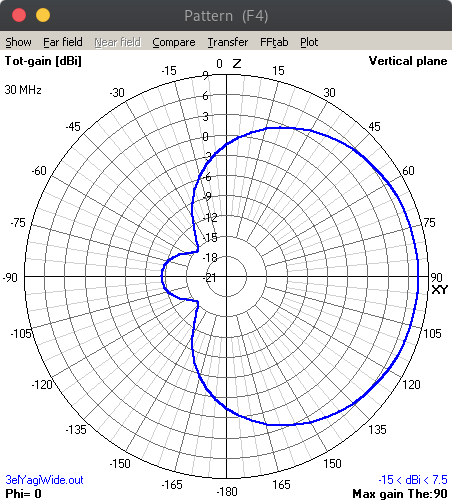
\includegraphics[scale=0.4]{images/Ejemplos/patern.png}
    \caption{El patrón de radiación de nuestra antena}
    \label{fig3:yagui2d}
\end{figure}

\begin{figure}[H]
    \centering
    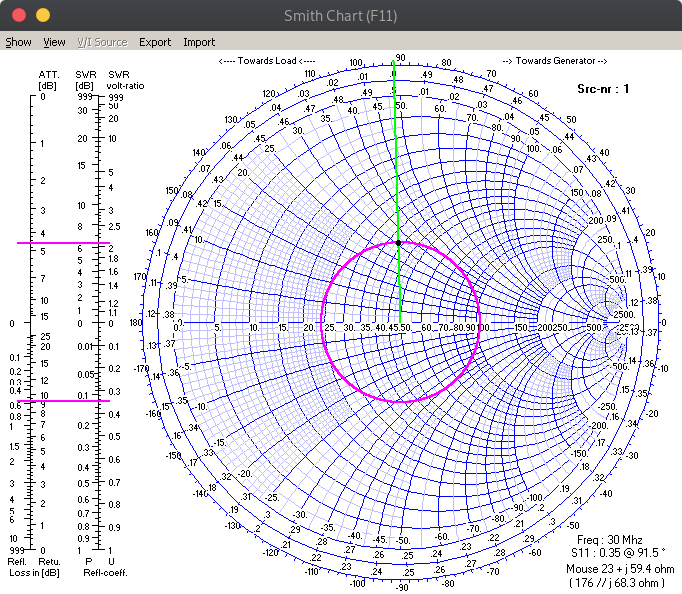
\includegraphics[scale=0.4]{images/Ejemplos/smith.png}
    \caption{Datos obtenidos plasmados en la carta de smith}
    \label{fig3:yagui2d}
\end{figure}

Como podemos observar nosotros necesitamos ingresar la frecuencia de trabajo y aplicar los métodos de verificación para saber que los resultados obtenidos en el main son correctos como se ve en el punto  \ref{sec:3.2} .\\
Aplicando el punto \ref{sec:3.2} de nuestro documento podemos decir que nuestro diseño es correcto y funcional ya que nuestra eficiencia es menor a 100\% pero es muy cercano debido a que no tiene cargas RLC, por otro lado también vemos que el valor de la impedancia es un valor realista mostrado en la ventana main, viendo el patrón de radiación podemos decir que es el comportamiento habitual de una antena yagi, y la energía también es la correcta, todo esto se puede comprobar en el programa y también siguiendo los cálculos teóricos desarrollados en clase.

Por otro lado en el programa podemos encontrar diferentes modelos de antenas que podemos usar, como también podemos diseñar, la interfaz de este programa es muy amigable y f\'acil de entender para poder diseñar.

\section{Ejemplo de diseño de una antena dipolo simple}\label{sec:6}
Se intenta diseñar una antena dipolo simple a una frecuencia de 30MHz, se debe tener en cuenta que para que una antena dipolo simple tiene una impedancia de 73$\Omega$

\textit{\textbf{Soluci\'on:}}
\begin{itemize}
    \item Lo primero que debemos realizar es el c\'alculo de nuestra longitud de onda ($\lambda$) de la siguiente manera:
\end{itemize}

\begin{align*}
    \lambda=\frac{c}{f}\\
    \lambda=\frac{3x10^8}{30x10^8}\\
    \lambda=10
\end{align*}


\begin{align*}
    d=\frac{\lambda}{2}\\
    d=\frac{10}{2}\\
    d=5
\end{align*}
    
Lo que nos da como resultado que cada brazo de nuestro dipolo medira 2.5m, este dato es importante para el diseño de nuestra antena 

Primera prueba diseñando nuestra antena dipolo:\\

\begin{itemize}
    \item Como primer punto ingresamos los datos en nuestra ventana de geometry edit
    
    \begin{figure}[H]
    \centering
    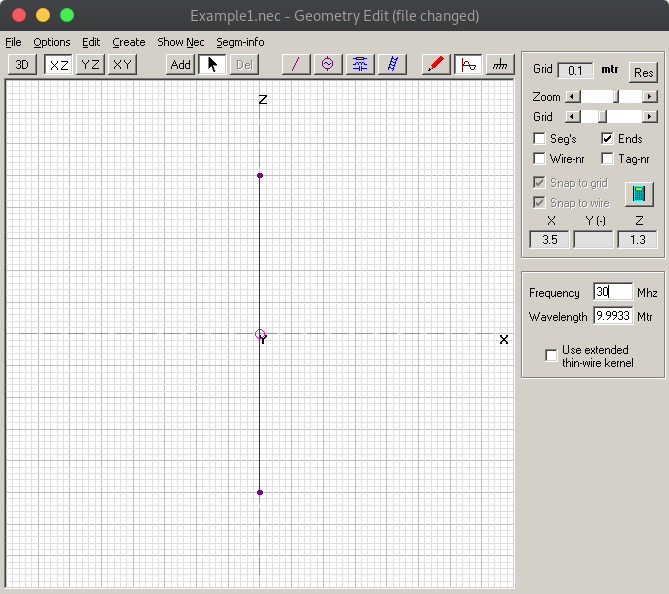
\includegraphics[scale=0.35]{images/dipolo/dipolo1.png}
    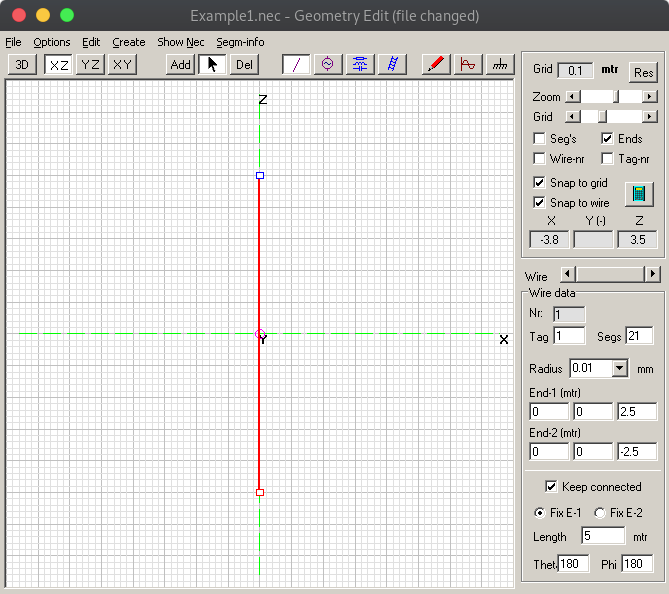
\includegraphics[scale=0.35]{images/dipolo/dipolo2.png}
    \caption{ingreso de los datos dados por el diseñador}
    \label{fig3:yagui2d}
    \end{figure}
    
\end{itemize}

Ahora una vez ingresado todos los datos necesarios, le damos a "Run NEC", que es la calculadora en la parte derecha de nuestra ventana, obteniendo los siguientes datos en la ventana main.

    \begin{figure}[H]
    \centering
    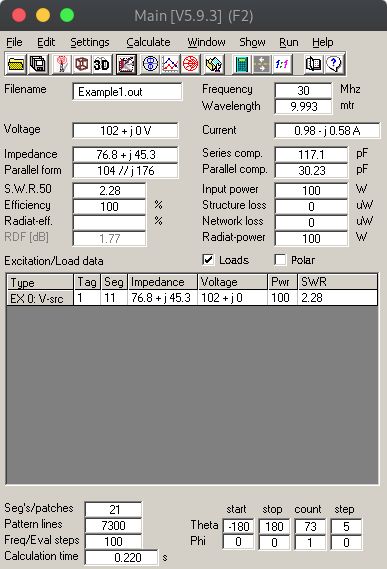
\includegraphics[scale=0.4]{images/dipolo/dipolomain.png}
    \caption{Datos obtenidos en el main}
    \label{fig3:yagui2d}
    \end{figure}
    
Se puede ver ya que nuestro diseño tiene error, debido a que la impedancia es mayor a 73

\begin{align*}
    76.8\Omega > 73\Omega
\end{align*}

Otro dato que nos indica que estamos en un error de diseño es que nuestro ROE o en su siglas en ingl\'es SWR, es mayor a 2, la que tenemos en nuestra simulaci\'on es de 2.28 y otro dato es nuestro coeficiente de reflexi\'on.

    \begin{figure}[H]
    \centering
    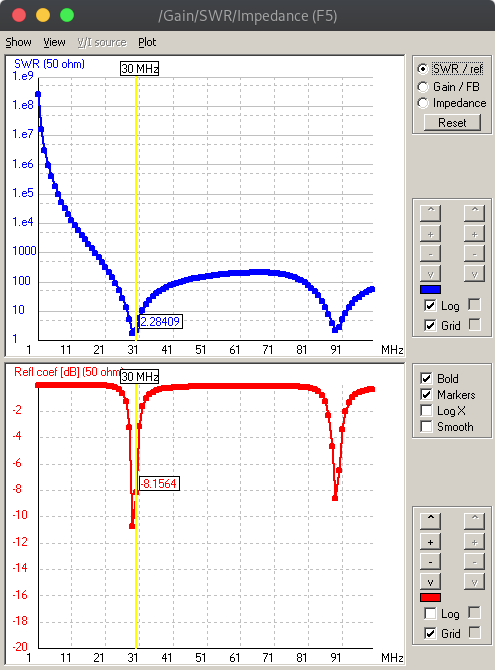
\includegraphics[scale=0.4]{images/dipolo/dipoloswr.png}
    \caption{Visualizaci\'on de coeficiente de reflexi\'on y SWR}
    \label{fig3:yagui2d}
    \end{figure}
    
Aqui ya observamos que nuestro coeficiente de reflexi\'on es mayor a -14dB, por lo cual nuestra antena es simplemente un error por lo que debemos modificar los valores ingresados.\\
Realizando diferentes pruebas modificando el valor del tamaño de nuestros brazos:

    \begin{figure}[H]
    \centering
    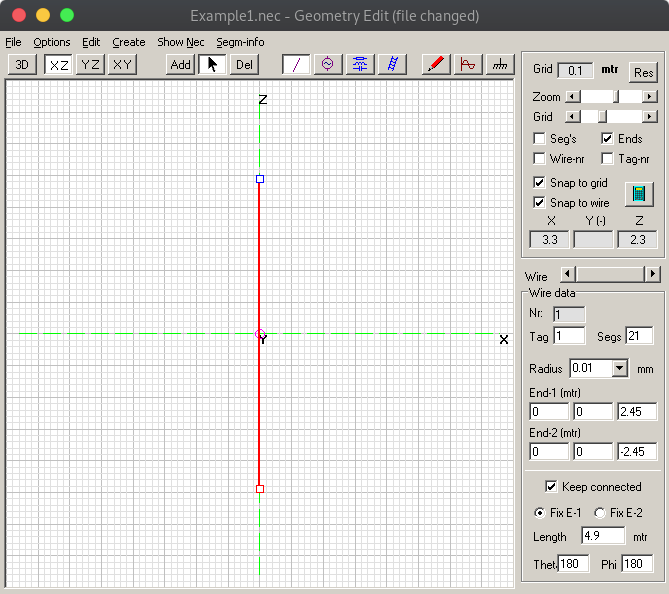
\includegraphics[scale=0.35]{images/dipolo/1dipolo.png}
    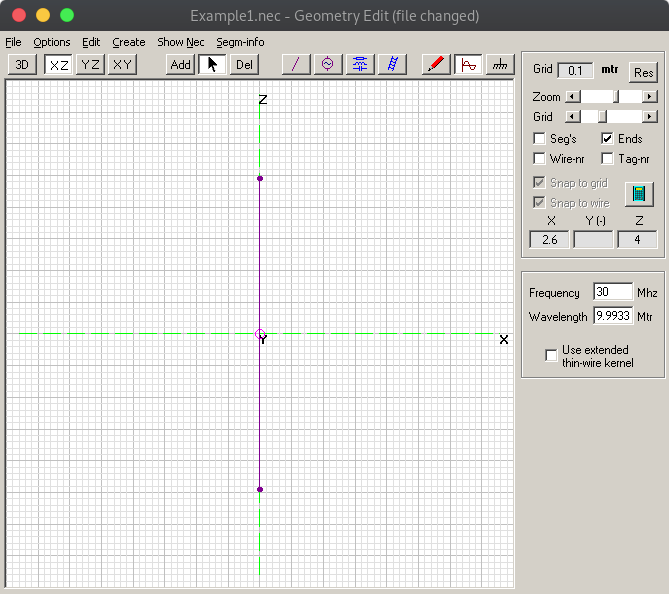
\includegraphics[scale=0.35]{images/dipolo/2dipolo.png}
    \caption{Datos modificados para obtener una antena dipolo factible}
    \label{fig3:yagui2d}
    \end{figure}

Obtenemos que con los valores anteriores nuestra antena ya est\'a lista para ser implementada y se corrobora su factibilidad viendo los siguientes datos

    \begin{figure}[H]
    \centering
    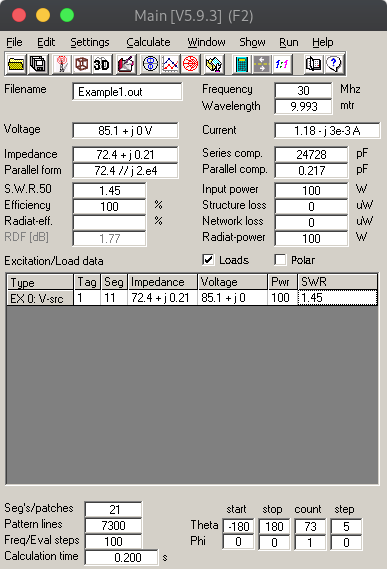
\includegraphics[scale=0.4]{images/dipolo/1dipolomain.png}
    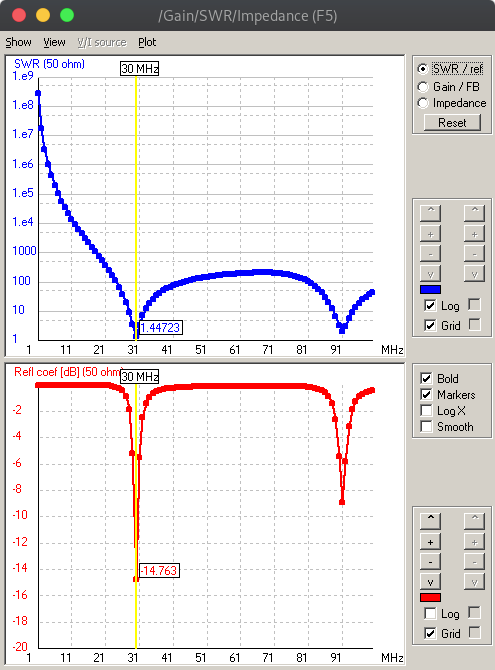
\includegraphics[scale=0.4]{images/dipolo/1dipoloswr.png}
    \caption{Comparaci\'on de datos}
    \label{fig3:yagui2d}
    \end{figure}

Comparando tenemos que 72.4$\lambda$ es muy cercano a 73$\lambda$ lo cual ya es un indicio, ahora nos fijamos que nues ROE es de 1.44, y como es menor a dos ya nos indica que nuestra antena es factible, y para sentirnos seguros nos fijamos que el coeficiente de refleci\'on es de -14.76dB, es decir que es menor a -14 dB as\'i que con estos datos estamos seguros de la implementaci\'on de nuestra antena que tiene un patr\'on de radiaci\'on:

    \begin{figure}[H]
    \centering
    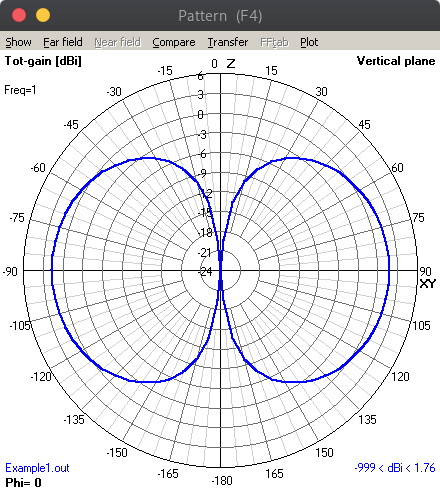
\includegraphics[scale=0.35]{images/dipolo/1pattern.png}
    \caption{Patr\'on de radiaci\'on de la antena dipolo simple implementada}
    \label{fig3:yagui2d}
    \end{figure}


\section{Conclusiones} 
\begin{itemize}
    \item Podemos obtener diferentes simulaciones y comportamientos de patrones de radiación en este programa de manera teórica por lo que nos da una idea de como será el comportamiento de nuestra antena de manera practica.
    \item Es una herramienta con un gran uso en el campo de las telecomunicaciones ya que podemos abarcar todo tipo de antenas ya sean dipolos, dipolos multi elemento, yagi, tipo parche, parab\'olicas, etc.
    \item Los resultados obtenidos en la ventana main nos puede dar una idea de si la implementación de nuestra antena será factible o no, con los respectivos valores de la eficiencia, los voltajes, las impedancias, etc. y también podemos percatarnos de eso viendo los resultados en la carta de smith que también te proporciona el programa.
    \item El programa funciona en un sistema operativo Windows, pero también puede ser usado en Linux con el problema de que no se puede visualizar el patrón de radiación y la misma antena en 3D.
\end{itemize}

\pagebreak
%\bibliographystyle{IEEEtranN}
\bibliographystyle{apalike}
\nocite{*}

\bibliography{bibliography}

\end{document}